
\chapter{Introduction}\label{ch:introduction}
System complexity is rising as systems engineering increasingly relies on digitally integrated and autonomous systems operating across expanding scopes and organizational boundaries \citep{incose2035}. Many contemporary systems no longer operate in isolation but cooperate with other independently managed systems to support shared objectives. In this setting, system of systems (SoS) describe configurations in which autonomous constituent systems coordinate their behaviour while retaining operational and managerial independence \citep{maier1998architecting}. SoS emphasize flexible coordination, loose coupling, and the ability for constituents to join, leave, or reorganize as objectives and operating conditions change, enabling collective behaviours that cannot be achieved by individual systems alone \citep{nielsen2015systems}.

In parallel, digital twins (DTs) have emerged as a means for achieving tight integration between physical systems and their digital representations. A DT maintains a bidirectional and continuously synchronized relationship with the system it represents, enabling observations from the physical world to update digital models and the analyses derived from them to influence physical operation \citep{kritzinger2018digital}. Through this digital--physical convergence, DTs support monitoring, simulation, prediction, and decision support across the system lifecycle \citep{pires2019digital, zhang2024digital, leng2021digital}.

\begin{figure}[t]
\centering
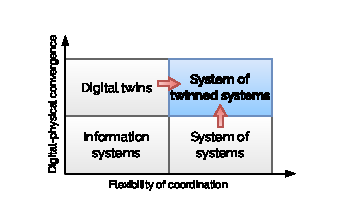
\includegraphics[width=0.75\linewidth]{figures/Introduction/quadrants-arrows.pdf}
\caption{SoTS coordination vs convergence.}
\label{fig:quadrants}
\end{figure}

By combining the flexible coordination principles of SoS engineering with the tight digital--physical coupling enabled by DTs, a new class of systems emerges, referred to as \emph{systems of twinned systems (SoTS)} \cite{adesanya2025systems}.

\begin{definitionframe}
A System of Twinned Systems (SoTS) comprises digitally twinned systems, i.e., digital and physical twins, organized by system of systems principles, in which digitally twinned systems may act as autonomous constituents and collaborate to achieve complex goals.
\end{definitionframe}

\paragraph{On the reliability of SoTS.}

SoTS form cooperative structures in which multiple autonomous DT enabled systems work together to achieve system-level objectives. DT based services support this cooperation by providing analytic capabilities that help interpret and reason about the behaviour of their physical counterparts. The effectiveness of these services depends on their ability to maintain correct reasoning as system conditions and constituent configurations evolve. The alignment that DTs maintain with their physical counterparts is inherently data-driven: DTs consume observations to update internal models and reason about system behaviour. As long as this flow of information remains consistent, these services can produce meaningful and correct outputs that reflect physical reality.

In SoTS, however, constituents operate in inherently dynamic environments. Systems may reconfigure, roles and responsibilities may change, sensing paths may differ over time, and communication conditions may fluctuate. As a result, the observations consumed by DTs may become incomplete or inconsistent, causing digital representations to diverge from the physical processes they are intended to reflect. Maintaining correct behaviour under such conditions is therefore a central reliability concern in SoTS.

Reliability, as defined by \citet{avizienis2004basic}, is the ability of a system to continuously deliver correct service. This definition emphasizes not only whether service is provided, but whether the results produced remain correct as operation progresses.
In the context of SoTS, this applies not only to physical constituents but also to DT based services that support monitoring, simulation, and analysis. The correctness of these services depends on maintaining alignment between digital representations and the evolving physical system, which in turn relies on the availability of observations produced by constituent systems. When observations are incomplete, maintaining correct reasoning becomes challenging, motivating the need for additional computational support that allows these services to remain correct under partial observational conditions.

\paragraph{Event-driven computation and complex event processing.}

In SoTS, the primary means by which DTs observe and track system behaviour is through discrete observations of state changes produced by their physical counterparts. These observations capture changes in system state as they occur and form the basis for updating digital representations over time. Reasoning about system behaviour and coordination is therefore organized around processing sequences of such observations, referred to as events \citep{luckham2002power}.

This processing is realized through complex event processing (CEP). CEP provides mechanisms for interpreting streams of observation events and detecting higher-level behaviours and patterns \citep{luckham2002power}. Conventional CEP approaches primarily define reasoning over events that are explicitly present in the input stream and focus on identifying patterns among observed occurrences. While existing extensions address uncertainty in observed values or temporal ordering, they offer limited support for reasoning about situations in which expected observations do not appear in the event stream \citep{alevizos2017probabilistic}. These limitations motivate the need for event-processing mechanisms that explicitly account for missing observations.

% ===========================
\paragraph{Thesis focus and approach.}
This thesis characterizes SoTS as an emerging class of systems formed through the coordination of DTs under SoS principles, and investigates the resulting reliability challenges. These challenges become most evident when expected observations are temporarily absent from event streams that support DT services.

The thesis therefore focuses on supporting reliable event-driven reasoning under partial data availability by addressing how the absence of observations is represented and handled during execution. The proposed approach introduces a formal model that defines expected observations, detects their absence at runtime, and reconstructs missing observations as events annotated with confidence values derived from state-based prediction. An accompanying architecture operationalizes this model within an event-driven processing pipeline, enabling downstream complex event processing engines to continue operating while explicitly accounting for the uncertainty introduced by inference and its impact on higher-level event detections.

% ====================================================
\section*{Research Contributions}
This thesis advances the understanding and operation of SoTS through the following contributions:

\textbf{Contribution 1 – Characterizing Systems of Twinned Systems and Their Reliability Gaps (\chref{ch:literature-review})} \\
Presents a systematic analysis of existing research to characterize systems of twinned systems as a distinct class of systems emerging from the integration of DTs and SoS principles. The analysis identifies recurring structural, architectural, and behavioural properties of SoTS and highlights a fundamental gap in existing work: while reliability is frequently recognized as an important concern, explicit mechanisms to address it are largely absent.


\textbf{Contribution 2 – A Formal Event Model and Architecture for Reliable Event-Driven Operation under Missing Observations (Chapters~\ref{ch:model} and~\ref{ch:architecture})} \\
Develops a formal model of event-driven computation that explicitly characterizes events, expected observations, and the absence of observations in event streams. Building on this model, the thesis introduces an architectural approach that detects missing observations, augments event streams with inferred events produced through state-based prediction, and propagates quantified uncertainty via confidence annotations.

\textbf{Contribution 3 – Implementation and Evaluation (Chapters~\ref{ch:implementation} and~\ref{ch:results})} \\
Implements the proposed model and architecture within a CEP-based processing pipeline and evaluates its behaviour under simulated data disruptions. The evaluation examines reconstruction accuracy, confidence evolution, and the impact of inferred events on higher-level pattern detection, demonstrating the feasibility and practical implications of the proposed approach for reliable event-driven processing.


% =======================================================
\vspace{1em}
Together, these contributions establish a foundation for reasoning about reliability in SoTS by situating reliability challenges at the level of event-driven computation and showing how partial data availability can be addressed within this setting. The remainder of the thesis develops this foundation by first grounding the work in relevant background and existing research (\chref{ch:background}, \chref{ch:literature-review}), then introducing a conceptual approach, formal event model, and supporting architecture for reasoning under missing observations (\chref{ch:approach}, \chref{ch:model}, \chref{ch:architecture}). The feasibility and implications of the approach are examined through implementation and evaluation (\chref{ch:implementation}, \chref{ch:results}), followed by a discussion of limitations, broader implications, and directions for future research (\chref{ch:discussion}, \chref{ch:conclusion}).

